\usetikzlibrary{arrows.meta}
\begin{frame}{running example}
\begin{itemize}
    \item based on Abramson, ``The Aloha System---Another alternative for computer comunications'' (1970)
    \vspace{.5cm}
    \item suppose we have shared radio with nodes A1, A2, \ldots, A$n$ and B
    \vspace{.5cm}
    \item A1, A2, \ldots A$n$ are all trying to transmit to B
    \item takes 1 ms to send message
    \item and want to collectively send $k$ messages per second
        \begin{itemize}
        \item randomly spaced (exponential distribution)
        \end{itemize}
\end{itemize}
\end{frame}

\begin{frame}{some probability}
    \begin{itemize}
    \item exponential distribution with mean $\lambda$
        \begin{itemize}
        \item our model for when packets sent
        \item ``memoryless'' distribution
        \item knowing when last packet sent tells you nothing about next
        \item (yes, not realistic)
        \end{itemize}
    \vspace{.5cm}
    \item probability events occur $< K$ time units apart \\
    $1-e^{-\lambda K}$
    \end{itemize}
\end{frame}


\begin{frame}{quiet time to avoid collisions}
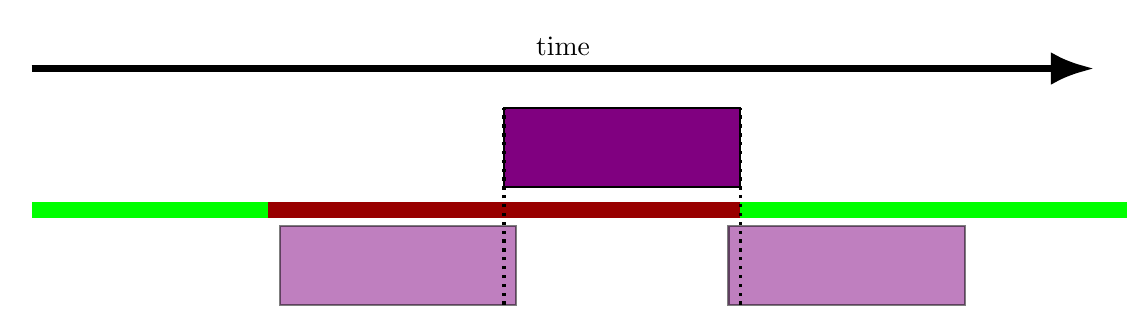
\begin{tikzpicture}
\begin{scope}[x=3cm]
    \draw[line width=1mm,-Latex] (-0.5, 0) -- (4, 0) node[above,midway] {time};
    \draw[thick,fill=violet] (1.5, -0.5) rectangle ++(1, -1);
    \draw[thick,fill=violet,opacity=0.5] (0.55, -2) rectangle ++(1, -1);
    \draw[thick,fill=violet,opacity=0.5] (2.45, -2) rectangle ++(1, -1);
    \path[fill=red!60!black] (0.5,-1.7) rectangle ++(2, -.2);
    \path[fill=green] (-0.5,-1.7) rectangle ++(1, -.2);
    \path[overlay,fill=green] (2.5,-1.7) rectangle ++(2, -.2);
    \draw[dotted,very thick] (1.5, -3) -- (1.5, -0.5);
    \draw[dotted,very thick] (2.5, -3) -- (2.5, -0.5);
\end{scope}
\end{tikzpicture}
\begin{itemize}
\item to avoid collision with 1 ms packet\ldots
\item can't start packet less than 1 ms before
\item can't start packet less than 1 ms after
\item $\rightarrow$ need 2 ms without packet starting for no collision
\end{itemize}
\end{frame}
% FIXME: diagram of 1.5 ms apart starts and collision

\begin{frame}{chance of collisions? (1)}
    \begin{itemize}
    \item to avoid collision when sending 1 ms packet
    \item need no other packet to be sent in 2ms period around its start time
    \vspace{.5cm}
    \item with $k$ packets/sec, chance is approx $1-e^{-\frac{2}{1000}k}$
    \end{itemize}
\end{frame}

\begin{frame}{chance of collision}
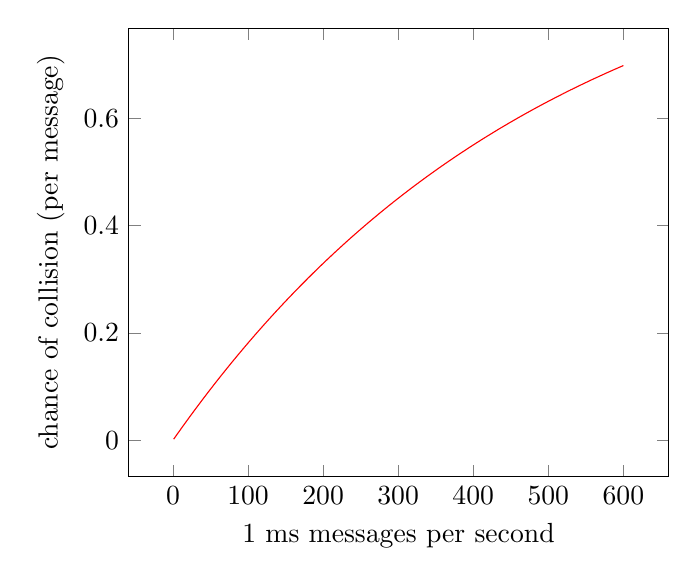
\begin{tikzpicture}
\begin{axis}[xlabel=1 ms messages per second,ylabel=chance of collision (per message)]
\addplot[domain=1:600,color=red,samples=1000]{1-exp(-(2 * x)/1000};
\end{axis}
\end{tikzpicture}
\end{frame}

\begin{frame}{retransmissions}
    \begin{itemize}
    \item what's going to happen when node can't send message
    \item probably it will retransmit it\ldots
    \vspace{.5cm}
    \item which means real transmission rate will be some $R > k$
        \begin{itemize}
        \item where $k$ is rate messages are generated
        \end{itemize}
    \item about $[1-e^{-2R\frac{1}{1000}}]$ chance of each message generated
    \item so $R = k + \left(1-e^{-2R\frac{1}{1000}}\right) \cdot R$
    \item $R = k + R - Re^{-2R\frac{1}{1000}}$
    \item $k = Re^{-2R\frac{1}{1000}}$
    \end{itemize}
\end{frame}

\begin{frame}{retranmissions (plot)}
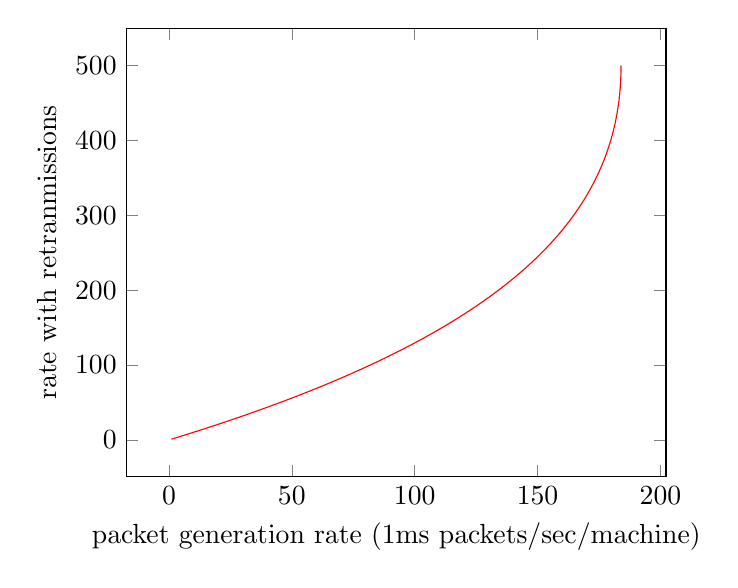
\begin{tikzpicture}
\begin{axis}[xlabel={packet generation rate (1ms packets/sec/machine)}, ylabel={rate with retranmissions}]
\addplot[domain=1:500,color=red,samples=1000] (x * exp(-2*x/1000), x);
\end{axis}
\end{tikzpicture}
\end{frame}

\begin{frame}{thinking about result}
    \begin{itemize}
    \item sending 500 1ms packet or retransmission/second
        \begin{itemize}
        \item using about half the capacity!
        \end{itemize}
    \item representing $\sim$ 186 1 ms non-retranmissions/second
        \begin{itemize}
        \item $\frac{1}{2e} = 0.186\ldots$
        \item using about 1/6th the capacity
        \end{itemize}
    \vspace{.5cm}
    \item results hold generally
    \item seems pretty bad for shared channel efficiency!
    \end{itemize}
\end{frame}
